\documentclass{standalone}
\usepackage{graphicx}	
\usepackage{amssymb, amsmath}
\usepackage{color}

\usepackage{tikz}
\usetikzlibrary{intersections, backgrounds}

\definecolor{light}{RGB}{220, 188, 188}
\definecolor{mid}{RGB}{185, 124, 124}
\definecolor{dark}{RGB}{143, 39, 39}
\definecolor{highlight}{RGB}{180, 31, 180}
\definecolor{gray10}{gray}{0.1}
\definecolor{gray20}{gray}{0.2}
\definecolor{gray30}{gray}{0.3}
\definecolor{gray40}{gray}{0.4}
\definecolor{gray60}{gray}{0.6}
\definecolor{gray70}{gray}{0.7}
\definecolor{gray80}{gray}{0.8}
\definecolor{gray90}{gray}{0.9}
\definecolor{gray95}{gray}{0.95}

\newcommand*{\offset}{0.025}

\begin{document}

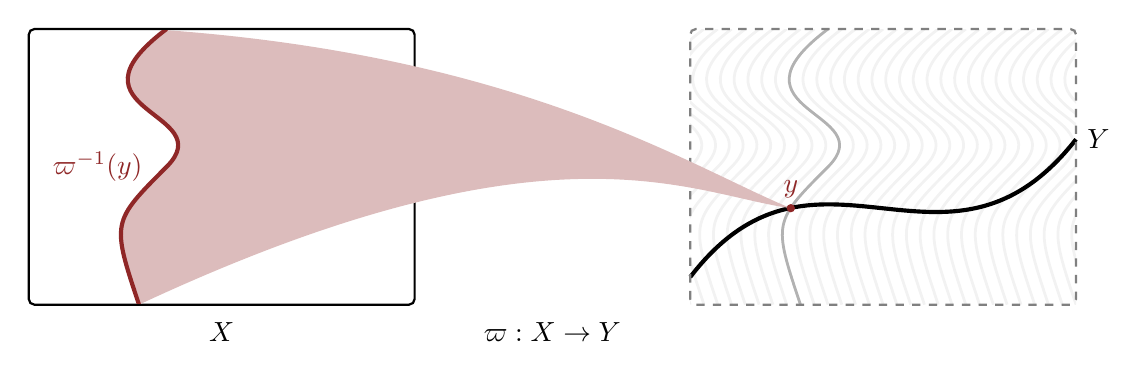
\begin{tikzpicture}[scale=0.35, thick]
  \draw [rounded corners=2pt, color=black] (-5, 0) rectangle +(-14, 10);
  \node at (-12, -1) { $X$ };
  
  \node at (0, -1) { $\varpi: X \rightarrow Y$ };
  
  \begin{scope}
    \clip (5, 0) rectangle +(14, 10);
    \foreach \i in {2.5, 3, ..., 21.5} {
      \draw [color=gray95, line width=1] (\i, 0) .. controls +(-1, 3) .. +(1, 5) .. 
                                         controls +(2, 2) and +(-4, -3) .. +(1, 10);
    }  
  \end{scope}
  
  \draw [color=gray70, line width=1] (9, 0) .. controls +(-1, 3) .. +(1, 5) .. 
                                     controls +(2, 2) and +(-4, -3) .. +(1, 10);
  
  \draw [line width=1.5] (5, 1) .. controls (9.6, 7) and (14.3, 0) .. (19, 6)
  node[right] { $Y$ };
  
  \draw [rounded corners=2pt, color=gray, dashed] (5, 0) rectangle +(14, 10);
  
  \fill [color=light] (-15, 0) .. controls +(-1, 3) .. +(1, 5) .. 
                     controls +(2, 2) and +(-4, -3) .. +(1, 9.96) ..
                     controls (-1, 9) and (5, 5) .. (8.65, 3.5) ..
                     controls (5, 4) and (0, 7) .. (-15, 0);
  
  \fill [fill=dark, text=dark] (8.65, 3.5) circle (0.15)
  node[above] { $y$ };
  
  \begin{scope}
    \clip (-5, 0) rectangle +(-14, 10);
    \draw [color=dark, line width=1.5] (-15, 0) .. controls +(-1, 3) .. +(1, 5) .. 
                                       controls +(2, 2) and +(-4, -3) .. +(1, 10);
  \end{scope}
  \draw (-9, 10) -- (-18, 10);
  \draw (-9, 0) -- (-18, 0);
  \node[color=dark] at (-16.5, 5) {$\varpi^{-1}(y)$};

\end{tikzpicture}

\end{document}  